\documentclass{article}

% if you need to pass options to natbib, use, e.g.:
% \PassOptionsToPackage{numbers, compress}{natbib}
% before loading nips_2017
%
% to avoid loading the natbib package, add option nonatbib:
% \usepackage[nonatbib]{nips_2017}

\usepackage[final]{nips_2017}

% to compile a camera-ready version, add the [final] option, e.g.:
%\usepackage[final]{nips_2017}

\usepackage[utf8]{inputenc} % allow utf-8 input
\usepackage[T1]{fontenc}    % use 8-bit T1 fonts
\usepackage{hyperref}       % hyperlinks
\usepackage{url}            % simple URL typesetting
\usepackage{booktabs}       % professional-quality tables
\usepackage{amsfonts}       % blackboard math symbols
\usepackage{nicefrac}       % compact symbols for 1/2, etc.
\usepackage{microtype}      % microtypography
\usepackage{amsmath}
\usepackage{graphicx}

\title{Machine Learning Based Graduate Admission Prediction}

% The \author macro works with any number of authors. There are two
% commands used to separate the names and addresses of multiple
% authors: \And and \AND.
%
% Using \And between authors leaves it to LaTeX to determine where to
% break the lines. Using \AND forces a line break at that point. So,
% if LaTeX puts 3 of 4 authors names on the first line, and the last
% on the second line, try using \AND instead of \And before the third
% author name.

\author{
  Tianbao Li\\
  Department of Computer Science\\
  University of Toronto\\
  Toronto, Ontario M5S 2E4\\
  \texttt{tianbao@cs.toronto.edu} \\
  %% examples of more authors
  %% \And
  %% Coauthor \\
  %% Affiliation \\
  %% Address \\
  %% \texttt{email} \\
  %% \AND
  %% Coauthor \\
  %% Affiliation \\
  %% Address \\
  %% \texttt{email} \\
  %% \And
  %% Coauthor \\
  %% Affiliation \\
  %% Address \\
  %% \texttt{email} \\
  %% \And
  %% Coauthor \\
  %% Affiliation \\
  %% Address \\
  %% \texttt{email} \\
}

\begin{document}
% \nipsfinalcopy is no longer used

\maketitle

\begin{abstract}
Graduation application to the US, Canada and the UK is a hot topic for students around the world, especially in China during the past years. Admission committee always gives out a final decision according to the student's background in many perspectives. Such decision can be considered as a classification problem and there is no much work on it by now. In this project, we applied several machine learning algorithms on our self-built dataset and trained models with relatively high accuracy.
\end{abstract}

\section{Introduction}

Nowadays, more and more Chinese students start to take graduate study overseas, usually in the US, Canada, the UK and somewhere else. Then, the problem just comes with it. How could they know whether a graduate school is going to offer admission or which one is the best fit?

Students usually finish their graduate application in two ways. The first one is to find an agency for help. Such agencies collect application data for year and give advice based on history cases and percentage on multiple indicators. However, misjudging always happens just because graduate admission consists of complex evaluation in many areas. The second type of application is called DIY-application, finished by students themselves. Due to lack of information, many students lose better offers.

During the application evaluation, information in many fields of one student is considered, including TOEFL score, GRE score, GPA and other supplementary materials as undergraduate school, work experience, research experience. Looking in the machine learning way, these indicators can be features of a certain model. We can use massive admission and rejection cases as training data and fit the admission model of a certain graduate program. Till now, decision for daily usage is mainly made by human experience in this area.

Comparing to human judgement and finding similar cases, many machine learning models seem to have a better prediction. A few related research built the process of decision making. \cite{raghunathan2010demystifying} and \cite{alzahranigot} give out the qualitative influence measurement on each part of the application material. Some work such as \cite{waters2014grade} is used to offer decision making assistance for universities. Work like \cite{bruggink1996statistical}, \cite{moore1998expert} and \cite{gupta2016will} use well-distributed data to build a statistic model and get good result. However, work like ours aims at producing a general prediction but not on a certain school. It means more valuable for applicants with multiple school choices. Also, the high quality data with great distribution that they use for certain universities is hard to get.

The contribution to this project is mainly is these points:

\begin{itemize}
    \item Dataset built-up: here I decide to use data from the BBS GTER\footnote{\url{http://bbs.gter.net/}}, one of the most popular graduate application BBSes in China. Many Chinese students post their admission decision here. I decide to write crawler to collection data of admission and rejection. Also due to the low data quality, much work on data cleaning needs to be done. Such data can be used for related purpose in the future research\\
    \item Model training: here I decide to train several popular machine learning models on such data, including neural networks, decision tree, naive bayes, etc, find better fit model and make optimization.\\
\end{itemize}

\subsection*{Clarification}

This project is finished by myself alone. With a self-defined dataset, some related work may continue on it afterwards.

\section{Data Summary}

Chinese students take a large portion in graduate application, however, there is no available dataset about it. So, for the first part of this project, we intent to built a dataset about Chinese student graduate application. We wrote web crawler to collect application data from GTER BBS, both admission and rejection application in the range of 2012-2016. Since web data usually holds low quality, some data cleaning skills are applied on the dataset to make it easy for model training.

Current dataset has 11056 cases. Due to natural language-based expression, the raw data is hard to catch related feature. Here, we only extract information about decision, target school, degree, year of application, TOEFL\footnote{\url{https://www.ets.org/toefl}} score, GRE\footnote{\url{https://www.ets.org/gre}} score, GPA, GPA ranking. Such information is transformed into 14 features and well normalized for training. Summary of the dataset is shown in Table~\ref{tab: Data_summary}.

\begin{table}[htbp]

\centering
    \begin{tabular}{cc}
        \textbf{General Information}\\
        \hline
        data point amount & 11056\\
        feature amount & 14\\
        \hline\\
        \textbf{Features for dataset}\\
        \hline
        result & admission:reject=4.48\\
        most popular school & Columbia University\\
        year range & [2012,2015]\\
        TOEFL total average & 84.8\\
        TOEFL reading average & 25.2\\
        TOEFL listening average & 22.1\\
        TOEFL speaking average & 23.1\\
        TOEFL writing average & 26.6\\
        GRE average & 319.0\\
        GPA average & 3.2\\
        \hline
    \end{tabular}

\caption{Data summary}
\label{tab: Data_summary}
\end{table}

\section{Prediction Models}

To predict whether a student will be admitted or rejected (binary classification), several models are trained and compared to get a relatively best model. From the direct perception of the data, in my opinion, decision tree should work well for the problem containing criterion of judgment, also KNN for same class data gathering together. So I also use a model simply combining decision tree and KNN together and try to get a promotion on accuracy. In the following section, we use $y$ to represent class variable and $\{x_1,x_2,\dots, x_n\}$ for features. All the models are implemented by scikit-learn\footnote{\url{http://scikit-learn.org/stable/}}.

\subsection{Naive Bayes}

Naive Bayes is a generative model based on Bayes’ theorem. Furthermore, it gives an assumption on features independency. It means that

$$
P(x_i|y,x_1,\dots,x_{i-1},x_{i+1},\dots,x_n)=P(x_i|y)
$$

so the decision rule is that

\newcommand{\argmax}{\operatornamewithlimits{argmax}}
$$
\hat{y}=\argmax_yP(y)\prod_{i=1}^nP(x_i|y)
$$

For implementation, we use MultinomialNB\footnote{\url{http://scikit-learn.org/stable/modules/generated/sklearn.naive_bayes.MultinomialNB.html}} from scikit-learn. To train a better fitting model, alpha (additive (Laplace/Lidstone) smoothing parameter) can be change as hyper-parameter.

\subsection{Logistic Regression}

Logistic regression is a linear classification model. Commonly, the model is optimized by minimizing the loss function (take l2 penalty as an example)

$$
min_{w,c}\frac{1}{2}w^\mathrm{T}w+C\sum_{i=1}^n\log(\exp(-y_i(X_i^\mathrm{T}w+c))+1)
$$

For implementation, we use LogisticRegression\footnote{\url{http://scikit-learn.org/stable/modules/generated/sklearn.linear_model.LogisticRegression.html}} from scikit-learn. In this model, hyper-perameters such as penalty (l1 or l2), C (inverse repolarization strength), tol (tolerance for stopping criteria) and some others can be changed.

\subsection{SVM}

Support Vector Machine is also a popular linear classification method with good performance. However, due to its advantages in high feature dimension, it is not expected to work so well for our scenario.

LinearSVC\footnote{\url{http://scikit-learn.org/stable/modules/generated/sklearn.svm.LinearSVC.html}} from scikit-learn. C (penalty parameter of the error term) is being monitored as hyper-parameter.

\subsection{KNN}

Distance-based K Nearest Neighbors is one suitable model for our problem. The first thought is that admitted cases hold the similar value on features, which means they are near in the feature space. It just fits the idea of nearest neighbors and it tends to work well.

For KNN, we use KNeighborsClassifier\footnote{\url{http://scikit-learn.org/stable/modules/generated/sklearn.neighbors.KNeighborsClassifier.html}} from scikit-learn as the model. Then we try to justify the hyper-parameter K (amount of neighbors) to have a higher accuracy.

\subsection{Decision Tree}

During the human admission process, it is usually divided into several decision rules, such as if the GPA high enough or if English using hits the criteria. Such process is similar to the decision tree classification. Also, the representative capability increases with the tree comes deeper.

In scikit-learn, DecisionTreeClassifier\footnote{\url{http://scikit-learn.org/stable/modules/generated/sklearn.tree.DecisionTreeClassifier.html}} can be used in this problem. For the hyper-parameter max\_depth, it could overfit when larger and underfit when smaller. So the parameter adjustment can be applied on this.

Futhermore, researchers usually use decision trees with much randomness, that is random forest. Comprised of several different decision trees, it often has better usually results on complex problem.

\subsection{Neural Networks}

As the most popular model, neural networks is solving quite different problems, linear or non-linear, simple or complex... Our project also play a easy try on this. MLPClassifier\footnote{\url{http://scikit-learn.org/stable/modules/generated/sklearn.neural_network.MLPClassifier.html}} is a non-GPU version implementation for small-scale application. Hyper-parameters of hidden layer sizes, activation functions are L2 penalty (regularization term) parameter are adjusting to achieve better.

\subsection{Combination of KNN and Decision Tree}

Following the discussion above, KNN and decision tree are the two models that could work well. To hold both advantages, here, we use a simple way to combine KNN and decision together (KNN-Tree).

First we train models of KNN and decision tree and get the class label as $y_{knn}$ and $y_{tree}$. Then a weighted sum (with $\alpha$) and threshold comparison (with $\beta$) work together to get the final label. That is

\begin{equation*}
    y=\left\{
    \begin{aligned}
        1,\quad & \alpha y_{knn}+(1-\alpha)y_{tree}>\beta\\
        0,\quad & \alpha y_{knn}+(1-\alpha)y_{tree}\le\beta
    \end{aligned}\right.
\end{equation*}

$\alpha$ and $\beta$ are selected as hyper-parameters.


\section{Experient Evaluation}

To evaluate the existing and proposed models, we try to use the self-built dataset and predict whether a student can be admitted by a university. To make a better use of the data, at first, we run data cleaning and normalization on the each feature and then calculate the accuracy for each model.

Detailed process of the project is introduced as follows. is shown as Figure~\ref{fig: Diagram}.

\begin{figure}[htbp]
\centering
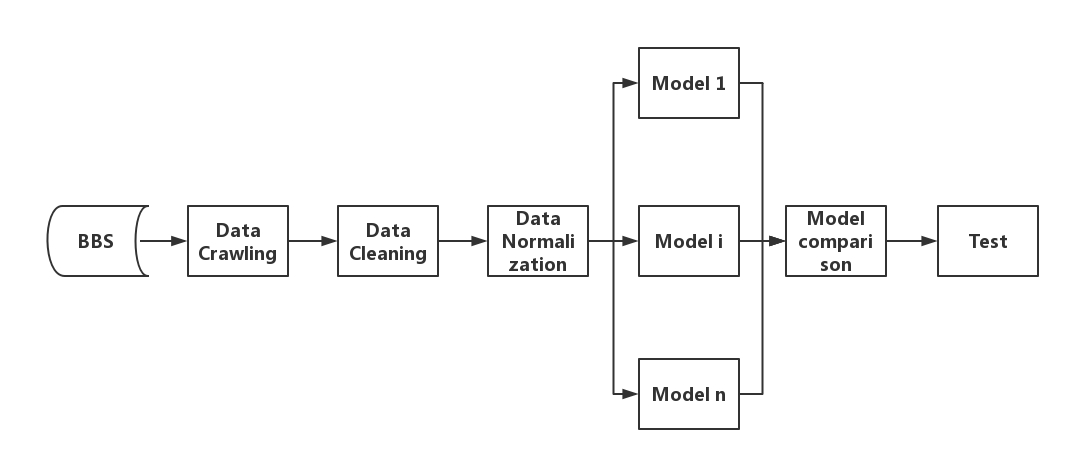
\includegraphics[width = 14cm]{Diagram}
\caption{System diagram}
\label{fig: Diagram}
\end{figure}

\subsection{Data Cleaning and Normalization}

As our dataset is crawled from web with human response, there should be a lot of errors or format inconsistent. To make use of it, the first thing to do is to clean the data and transform the information to the feature that we need. Also, normalizing the data into a similar range can help models work better.

Data cleaning on this dataset contains:

\begin{itemize}
    \item natural language extraction: there is some information in the inexplicit natural language words as admission result. Some rules are written for this.
    \item inconsistency: some information are inconsistent among cases like university name. Regularization work lile string fuzzy matching is needed for this. Here we use python package FuzzyWuzzy\footnote{\url{https://github.com/seatgeek/fuzzywuzzy}} and match user input with common-used university name.
    \item missing value filling: due to some reason, some cases lack of TOEFL or GRE value. For keeping the influence to a lowest range, we fill them with average value for each.
    \item data format: the raw data is in csv format, with many commas as a part of values. The data is well-split and transformed into json file finally.
\end{itemize}

Data normalization on the dataset contains:

\begin{itemize}
    \item university: university name is a non-numerical value and hard for training. we use university ranking from Times\footnote{\url{https://www.timeshighereducation.com/world-university-rankings}} and replace the university name. Normally, highly ranked universities have high admission requirement.
    \item degree: 1 for master and 2 for Ph.D
    \item application year: map year [2012,2013,2014,2015] into[0.00,0.25,0.50,0.75]. (leave 2016 to 1 behind for future extension)
    \item decision result: 0 for rejection and 1 for admission (only admission and offer)
    \item TOEFL score: change total score [0,120] into [0,1] and sub-score from [0,30] into [0,1] by division.
    $$
    total\_normalized=total/120
    $$
    $$
    sub\_normalized=sub/30
    $$
    \item GRE score: change total score [260,340] into [0,1], Verbal/Quantitative score from [130,170] into [0,1] and writing score from [0,6] into [0,1] by division.
    $$
    total\_normalized=(total-260)/80
    $$
    $$
    sub\_normalized=(sub-130)/40
    $$
    $$
    writing\_normalized=writing/6
    $$
    \item GPA: most cases have GPA score in the form of 4.0-total or 100-total. Just turn them into [0,1] by official method.
    \item GPA ranking: transforming into percentile
\end{itemize}

\subsection{Evaluation Metrics}

Evaluation used in the project is one of the most simple but effective, accuracy. It is shown as this:

$$
accuracy=\frac{hits}{total}
$$

\subsection{Model Comparison}

For model comparison, we split the dataset into training data and test data, which test data holds the percentage of 20\%. Also for model training, 20\% of training data is for validation and hyper-paramater choosing.

The detailed train accuracy, test accuracy are shown in Table~\ref{tab: Model_comparison}.

\begin{table}[htbp]
\centering
\begin{tabular}{cccc}
    \hline
    Model & Train accuracy & test accuracy\\
    \hline
    MultinomialNB & 0.568401371144 & 0.549190535492\\
    \hline
    Logist Regression & 0.620442505453 & 0.683483802443\\
    \hline
    SVM & 0.620442505453 & 0.626400996264\\
    \hline
    KNN & 0.998753505765 & 0.765877957659\\
    \hline
    Decision Tree & 0.999065129324 & 0.752179327522\\
    \hline
    Random Forest & 0.999065129324 & 0.753424657534\\
    \hline
    Neural Networks & 0.616703022749 & 0.59900373599\\
    \hline
    KNN+Decision Tree &  & 0.789539227895\\
    \hline
    \end{tabular}
\caption{Model comparison}
\label{tab: Model_comparison}
\end{table}

From the result of the accuracy, best performed existing models are KNN Decision Tree and Random Forest. What's more, out proposed combination model of KNN and Decision Tree improves the accuracy by 2-3 percentage.

\section{Future Work}

Due to the time of a final project, the proposed problem was just solved simply with a relatively good result. However, for a prediction that could make value, more work could be done in the future, including

\begin{itemize}
    \item our models only concentrate on global admission, but not a certain university of even graduate program. When more specific data is collected, out system can also do the work like \cite{bruggink1996statistical}, \cite{moore1998expert} and \cite{gupta2016will}.
    \item only part of the information we get is used for model training. Hope more skills can be used to deal with natural-languaged info like research outcome, internship experience, awards and transform them into well-scaled features.
    \item for the project we only use some existing algorithms and propose one simple combination of well-performed ones. More complex can apply on this problem, especially neural networks.
    \item also based on what we have done, application recommendation on university can be made as a similar regression problem (on university ranking range) that values much.
\end{itemize}

\section{Conclusion}

This paper introduces the project for make prediction on graduate admission in machine learning methods. Our goal is to give out application assistance for students on whether he/she will be admitted by a university. We collected from true BBS data and made it as a well-organized dataset. Then we trained several existing algorithms and combined two well-performed models. The KNN with Decision Tree model has an accuracy of 79.0\% on test set which can be a part of application assistance. By opening the self-built dataset, hope more work could be done on this problem.

\bibliographystyle{plain}
\bibliography{CSC2515_Report_TianbaoLi}

\end{document}
